\documentclass[11pt]{standalone}
\usepackage{amssymb}
\usepackage{amsmath}
\usepackage[no-math]{fontspec}
\usepackage{unicode-math}
\usepackage{libertinus}
\usepackage{pgf,xcolor}
\usepackage{tikz}
\usetikzlibrary{arrows.meta, backgrounds}
\usepackage{pgfplots}
\pgfplotsset{compat=newest}

\definecolor{my_darkgray}{HTML}{484949}
\definecolor{my_lightgray}{HTML}{F3F4F4}
\definecolor{my_darkblue}{HTML}{005A94}
\definecolor{my_lightblue}{HTML}{CCDEE9}
\definecolor{my_yellow}{HTML}{FFEC7F}
\definecolor{my_red}{HTML}{E60000}
\definecolor{my_orange}{HTML}{E87846}

\begin{document}

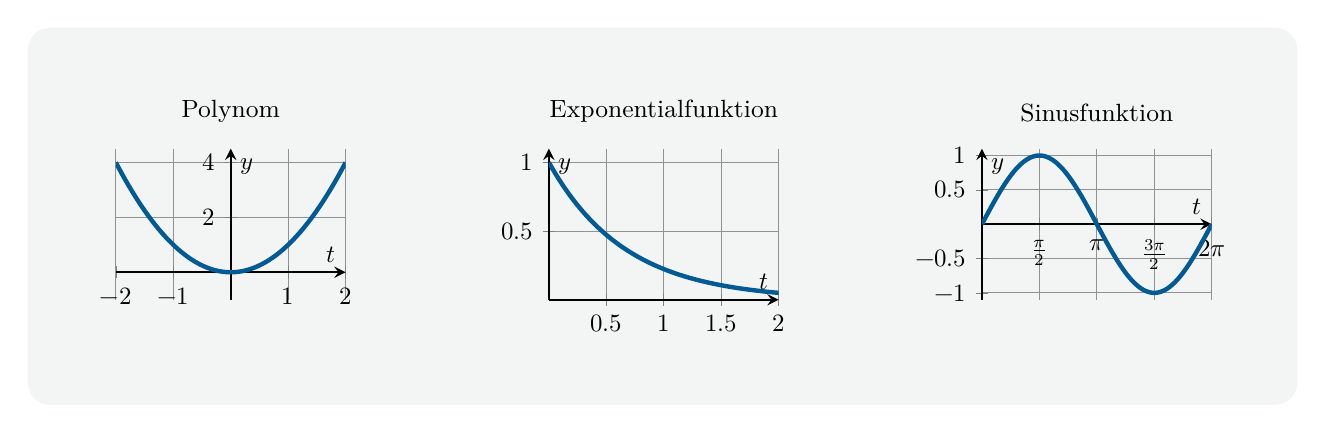
\begin{tikzpicture}[
    show background rectangle,
    background rectangle/.style={fill=my_lightgray, rounded corners=8pt},
    inner frame sep=0.8cm
]

% --- Panel 1: Polynom -----------------------------------------------
\begin{axis}[
    width = 4.5cm,
    height = 3.5cm,
    xshift = 0cm,
    axis lines = center,
    axis line style = {thick},
    xlabel = {$t$},
    ylabel = {$y$},
    xlabel style = {font=\small},
    ylabel style = {font=\small},
    ticklabel style = {font=\small},
    grid = both,
    minor grid style = {draw=my_lightblue},
    major grid style = {draw=my_darkgray!60},
    xmin = -2,
    xmax = 2,
    ymin = -1,
    ymax = 4.5,
    title = {Polynom},
    title style = {font=\small},
    % axis equal hier bewusst weggelassen, damit der Verlauf gut erkennbar ist.
]

\addplot[
    draw = my_darkblue,
    ultra thick,
    samples = 300,
    domain = -2:2
]
{x^2};

\end{axis}

% --- Panel 2: Exponentialfunktion -----------------------------------
\begin{axis}[
    width = 4.5cm,
    height = 3.5cm,
    xshift = 5.5cm,
    axis lines = center,
    axis line style = {thick},
    xlabel = {$t$},
    ylabel = {$y$},
    xlabel style = {font=\small},
    ylabel style = {font=\small},
    ticklabel style = {font=\small},
    grid = both,
    minor grid style = {draw=my_lightblue},
    major grid style = {draw=my_darkgray!60},
    xmin = 0,
    xmax = 2,
    ymin = 0,
    ymax = 1.1,
    title = {Exponentialfunktion},
    title style = {font=\small},
    % axis equal hier bewusst weggelassen, damit der Abfall sichtbar bleibt.
]

\addplot[
    draw = my_darkblue,
    ultra thick,
    samples = 300,
    domain = 0:2
]
{exp(-1.5*x)};

\end{axis}

% --- Panel 3: Sinusfunktion -----------------------------------------
\begin{axis}[
    width = 4.5cm,
    height = 3.5cm,
    xshift = 11.0cm,
    axis lines = center,
    axis line style = {thick},
    xlabel = {$t$},
    ylabel = {$y$},
    xlabel style = {font=\small},
    ylabel style = {font=\small},
    ticklabel style = {font=\small},
    grid = both,
    minor grid style = {draw=my_lightblue},
    major grid style = {draw=my_darkgray!60},
    xmin = 0,
    xmax = 2*pi,
    ymin = -1.1,
    ymax = 1.1,
    xtick = {0, 1.5708, 3.1416, 4.7124, 6.2832},
    xticklabels = {$0$, $\frac{\pi}{2}$, $\pi$, $\frac{3\pi}{2}$, $2\pi$},
    title = {Sinusfunktion},
    title style = {font=\small},
    % axis equal hier bewusst weggelassen, um den Verlauf gut zu erkennen.
]

\addplot[
    draw = my_darkblue,
    ultra thick,
    samples = 300,
    domain = 0:2*pi
]
{sin(deg(x))};

\end{axis}

\end{tikzpicture}

\end{document}